\section{Optimalizačné metódy}
\label{se:optimalizacia}

V tejto časti teórie si rozoberieme optimalizačné metódy, ktoré budeme využívať v rámci tejto práce. Ako prvé sa pozrieme na numerickú optimalizáciu, pomocou ktorej budeme získavať riešenie pre naše optimalizačné problémy. V druhej časti si ukážeme metódu pre decentralizovanú optimalizáciu, vďaka ktorej budeme schopný rozložiť si MPC na $N$ predikčných horizontov a následne ich optimlaizovať samostatne. 
\subsection{Analitická optimalizácia}


\subsection{Numerická optimalizácia}
Keďže budeme využívať numerickú optimalizáciu len pre optimalizáciu prediktívneho regulátora máme vždy k dispozícií predpis optimalizovanej účelovej funkcie čiže aj jej gradient. Preto sa nám ponúka k dispozícií numerická optimalizácia založená na gradiente účelovej funkcie. 

Základnou metódou je Gradientová metóda, ktorá využíva gradient k nájdeniu optima. V našom prípade budeme chcieť minimalizovať účelovú funkciu a tak sa budeme pohybovať v smere poklesu gradientu. Jedná sa o takzvanú lokálnu metódu, čiže pri nekonvexných optimalizačných problémoch môže uviaznuť v lokálnom minime. Avšak MPC je kvadratický optimalizační problém teda má konvexnú účelovú funkciu, ktorá má práve jednu hodnotu lokálneho minima a ľahko sa optimalizuje. 

\begin{figure}[H]
	\centering
	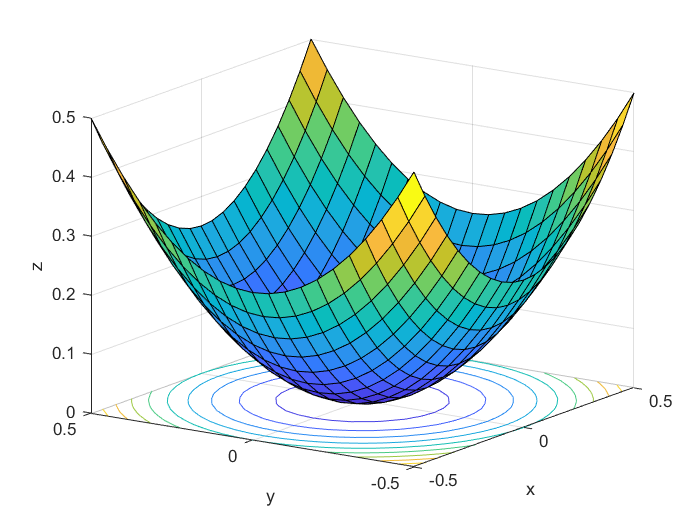
\includegraphics[width=7cm,height=5cm]{images/Konvexna_funkcia}
	\caption{Konvexná účelová funkcia}
\end{figure}

Gradientová metóda sa rieši pomocou nasledovných krokov
\begin{description}
	\item[Krok 1:] {Zvolíme si začiatočný bod $x$}
	\item[Krok 2:] {Zavoláme gradient funkcie $\nabla f(x)$}
	\item[Krok 3:] {Vypočítame smer poklesu $\Delta x = -\nabla f(x)$}
	\item[Krok 4:] {Pomocou backtracking nájdeme vhodný krok $t$ a aktualizujeme optimalizované premenné $x = x + \Delta x $}
	\item[Krok 5:] {Opakujeme od kroku č.2 až kým nenarazíme na zastavovacie kritéria}
\end{description}


\subsection{Decentralizovaná optimalizácia}